\section{Mathematische Grundlagen}

\textbf{Kinematik} ist die reine geometrische Beschreibung von Bewegung eines Manipulators
oder Roboters. Das essentielle Konzept ist die \textbf{Position}.

\textbf{Statik} behandelt Kräfte und Momente, die sich auf einen ruhenden Mechanismus
auswirken. Das essentielle Konzept ist die \textbf{Steifigkeit}.

\textbf{Dynamik} analysiert die Kräfte und Momente, die durch Bewegung und Beschleunigung
eines Mechanismus und einer zusätzlichen Last entstehen.

\textbf{Freiheitsgrade} (DoF) ist die Anzahl unabhängiger Parameter, die zur kompletten Spezifikation der Lage eines Objekts benötigt werden, z.B. Starrkörper hat in 2D 3 DoF und in 3D 6 DoF.

\textbf{Starrkörperbewegungen werden durch zwei Eigenschaften charakterisiert}:
\begin{enumerate}
	\item Distanz zweier beliebiger Punkte ist konstant
	\item Orientierungen im Körper bleiben erhalten
\end{enumerate}

\textbf{SO(3) und SE(3)}:
\begin{itemize}
	\item SO(3): \textbf{Spezielle Orthogonale Gruppe}, die \textbf{Rotationen} repräsentiert
	\item SE(3): \textbf{Spezielle Euklidische Gruppe}, die \textbf{Transformationen} repräsentiert
	\item Elemente aus SO(3) werden als reale $3\times3$ orthogonale Matrizen $R$ (Zeilen- und Spaltenvektoren orthonormal) beschrieben und erfüllen
	$$R^\top R=1 \qquad \text{ mit } \qquad\det(R)=1$$
	\item Elemente aus SE(3) sind von der Form $(\mathbf{p},R)$ mit $\mathbf{p}\in\R^3$ und $R\in\text{SO(3)}$ und beschreiben Verknüpfungen von Rotationen und Translationen
	\begin{center}
		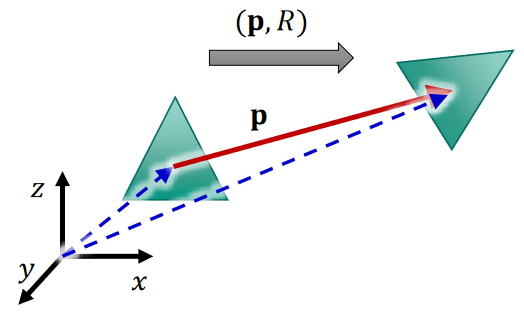
\includegraphics[width=0.4\textwidth]{images/se3.png}
	\end{center}
\end{itemize}
\medskip
\textbf{Euklidischer Raum}: Vektorraum $\R^3$ mit dem Skalarprodukt.
\begin{itemize}
	\item Punkt $\mathbf{a}$ im euklidischen Raum wird durch Vielfache der Einheitsvektoren $\mathbf{e_x}, \mathbf{e_y}, \mathbf{e_z}$ beschrieben
	\item Wir benutzen \textbf{rechtsdrehende Koordinatensysteme}
\end{itemize}
\begin{center}
	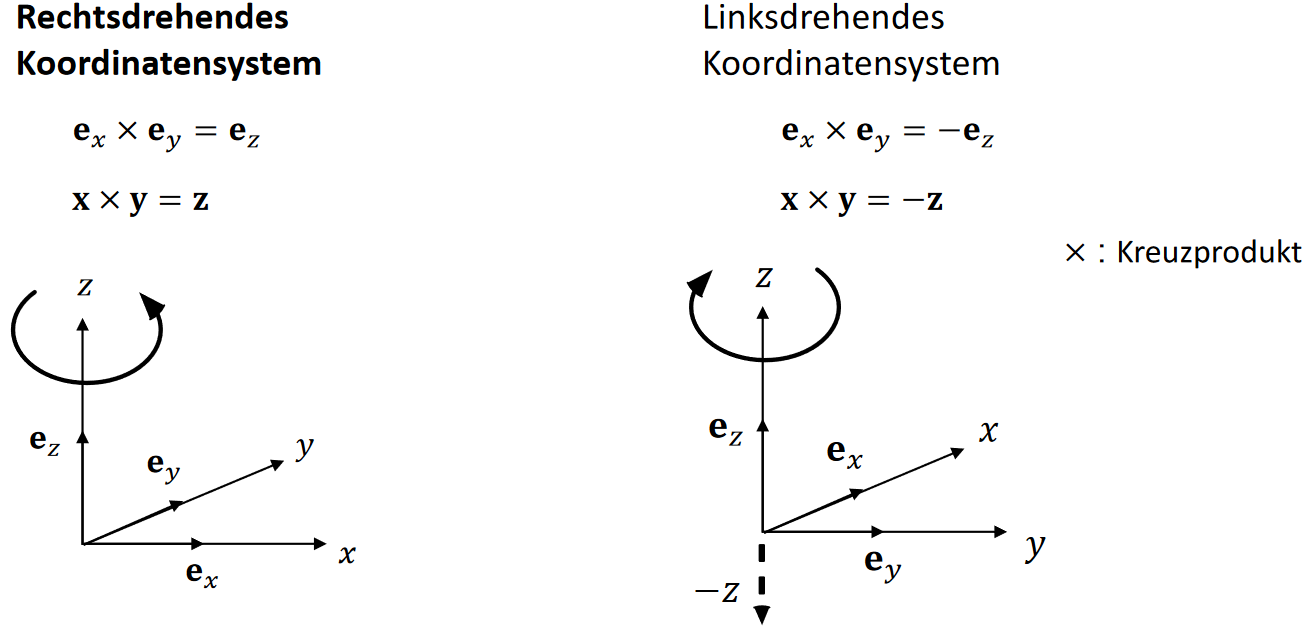
\includegraphics[width=0.75\textwidth]{images/koordinaten.png}
\end{center}
\medskip
\textbf{Lineare Abbildungen}  (Transformationen), die den euklidischen Raum auf sich selbst abbilden, nennt man \textbf{Endomorphismen}: $$\phi(\cdot)\colon\R^3\rightarrow\R^3$$
\begin{itemize}
	\item Endomorphismen können durch quadratische Matrizen repräsentiert werden: $$\phi(\mathbf{a})=A\cdot\mathbf{a},\qquad A\in R^{3\times 3}$$
	\item $A$ beschreibt einen Basiswechsel zwischen den originalen Basisvektoren $\mathbf{e_x}, \mathbf{e_y}, \mathbf{e_z}$ und den neuen Basisvektoren $\mathbf{e_x'}, \mathbf{e_y'}, \mathbf{e_z'}$:
	
	$$A=\irow{\mathbf{e_x'}&\mathbf{e_y'}&\mathbf{e_z'}}\cdot\irow{\mathbf{e_x}&\mathbf{e_y}&\mathbf{e_z}}^{-1}$$
\end{itemize}

\textbf{Bijektive} Endomorphismen nennt man \textbf{Isomorphismen}.
\begin{itemize}
	\item Eigenschaften:
	\begin{enumerate}
		\item Winkel bleiben erhalten
		\item Längen bleiben erhalten
		\item Händigkeit beleibt erhalten
	\end{enumerate}
	\item Eine spezielle Art von Isomorphismen ist die \textbf{Rotationsgruppe} SO(3)
\end{itemize}
\medskip
\textbf{Rotationsgruppe SO(3):}
\begin{itemize}
	\item SO(3) ist nicht kommutativ: $A\cdot B\cdot \mathbf{x}\neq B\cdot A\cdot \mathbf{x}$ mit $\mathbf{x}\in\R^3$ und $A,B\in\text{SO(3)}$ 
	\item Für alle $R\in\text{SO(3)}$ ist $R^{-1}=R^\top$, die Inverse kann also leicht berechnet werden
\end{itemize}
\pagebreak
\textbf{Rotationen in 2D}:
\begin{itemize}
	\item Rotation in der $xy$-Ebene um $(0,0)$ ist eine \textbf{lineare Transformation}
	\item \textbf{Rotationsmatrix}: $R_\alpha(\mathbf{x})=
	\left(\begin{matrix}
		\cos\alpha & -\sin\alpha \\
		\sin\alpha & \cos\alpha 
	\end{matrix}\right)\cdot\mathbf{x}$
	mit $RR^\top=R^\top R=I$ und $\det(R)=1$
	\item Rotation um einen Punkt $\mathbf{c}\neq(0,0)$ ist keine lineare Transformation.
	Verschiebe dafür die Ebene um $-\mathbf{c}$, rotiere und verschiebe wieder um $+\mathbf{c}$ zurück:
	$$R_{\mathbf{c},\alpha}=R_\alpha(\mathbf{x}-\mathbf{c})+\mathbf{c}= R_\alpha(\mathbf{x})+(-R_\alpha(\mathbf{c})+\mathbf{c})$$
	\item $R_{\mathbf{c},\alpha}$ ist eine nichtlineare Transformation und heißt \textbf{affine Transformation}.
	Sie unterscheidet sich von $R_\alpha$ nur durch das Addieren einer Konstante
\end{itemize}
\medskip
\textbf{Rotationen in 3D}:
\begin{itemize}
	\item Eine 2D Rotation in der $xy$-Ebene ist eine 3D Rotation um die $z$-Achse: $$R_{\mathbf{z},\alpha}=\left(\begin{matrix}
		\cos\alpha & -\sin\alpha & 0 \\
		\sin\alpha & \cos\alpha & 0 \\
		0 & 0 & 1
	\end{matrix}\right)$$
	\item Rotationen können verkettet werden: $\phi_{\mathbf{z},\gamma}\left(\phi_{\mathbf{y},\beta}\left(\phi_{\mathbf{x},\alpha}(\mathbf{a})\right)\right),\qquad \mathbf{a}\in\R^3$
\end{itemize}
\medskip
\textbf{Probleme mit Rotationsmatrizen}:
\begin{itemize}
	\item \textbf{Redundanz}: Neun Werte für eine Rotationsmatrix
	\item Probleme im Bereich des maschinellen Lernens
\end{itemize}
\bigskip
\textbf{Eulerwinkel}:
\begin{itemize}
	\item Es ist möglich jede Rotation durch drei Rotationen um jeweils eine Rotationsachse darzustellen
	\item \textbf{Euler-Konvention}: $\mathbf{z}\text{ }\mathbf{x'}\text{ }\mathbf{z''}$ (lokale Drehung, Drehung verändert Achsen) oder $\mathbf{x}\text{ }\mathbf{y}\text{ }\mathbf{z}$ (globale Drehung, Drehung um feste Achsen)
	\item Winkel $\alpha,\beta,\gamma$ sind \textbf{Eulerwinkel} und beschreiben den Grad der Drehungen
	\begin{center}
		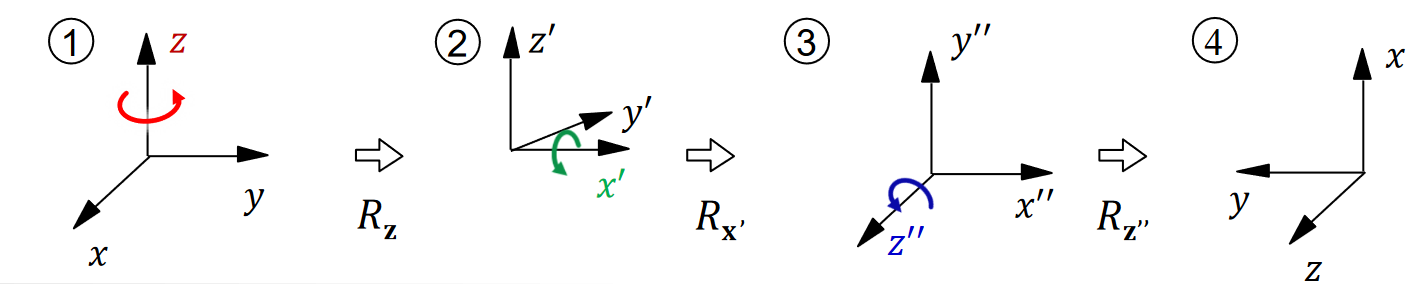
\includegraphics[width=0.7\textwidth]{images/euler.png}
	\end{center}
	\item \textbf{Vorteile}: Kompakter und aussagekräftiger als Rotationsmatrizen
	\item \textbf{Nachteile}: 
	\begin{itemize}
		\item Nicht eindeutig: In der Euler-Konvention $\mathbf{x}\text{ }\mathbf{y'}\text{ }\mathbf{z''}$ beschreiben die Eulerwinkel $(45^\circ,-90^\circ,45^\circ)$ und 
		und $(30^\circ,-90^\circ,60^\circ)$ die gleiche Rotation
		\item Nicht kontinuierlich: Kleine Änderung in der Orientierung können zu großen Änderungen der Eulerwinkel führen
		\item \textbf{Gimbal Lock}: Bei bestimmten Winkeln werden zwei Achsen voneinander abhängig $\Rightarrow$ Ein Freiheitsgrad geht verloren
	\end{itemize}
\end{itemize}
\bigskip
\textbf{Bewertung der Darstellung von Orientierung mit $\mathbf{3\times3}$-Matrizen}:
\begin{itemize}
	\item \textbf{Vorteil}: Vektor und Rotationsmatrix sind anschaulich $\Rightarrow$ übliche Form der Eingabe von Posen
	\item \textbf{Nachteil}: Darstellung als $(\mathbf{p},R)$ mit $\mathbf{p}\in\R^3$ und $R\in\text{SO(3)}$ führt dazu, dass Translation und Rotation getrennt durchgeführt werden müssen 
\end{itemize}

$\rightarrow$ \textbf{Ziel}: Geschlossene Darstellung von Rotation und Translation in einer Matrix\\

\textbf{Affine Transformationen}:
\begin{itemize}
	\item Der \textbf{affine Raum} ist eine Erweiterung zum euklidischen Raum
	\item Beinhaltet Vektoren, die in \textbf{erweiterten, homogenen Koordinaten} ausgedrückt werden: $a=\irow{a_x&a_y&a_z&h}^\top, h\in\{0,1\}$, wobei $a$ für $h=0$ einen Ortsvektor und für $h=1$ einen Richtungsvektor beschriebt
	\item Für Rotationsmatrix $R$ und Translation $\mathbf{t}$ gilt nun: 
	$$\mathbf{b}=A\cdot\mathbf{x}+\mathbf{t}
	\Leftrightarrow 
	\left(\begin{matrix}
		\mathbf{b} \\
		1
	\end{matrix}\right)=
	\left(\begin{matrix}
		A & \mathbf{0} \\
		\mathbf{0}^\top & 1
	\end{matrix}\right)
	\left(\begin{matrix}
		\mathbf{x} \\
		1
	\end{matrix}\right)+
	\left(\begin{matrix}
		\mathbf{t} \\
		0
	\end{matrix}\right)=
	\left(\begin{matrix}
		A & \mathbf{t} \\
		\mathbf{0}^\top & 1
	\end{matrix}\right)
	\left(\begin{matrix}
		\mathbf{x} \\
		1
	\end{matrix}\right)
	$$
	womit also nun Translation und Rotation als eine allgemeine homogene $4\times4$-Matrix beschrieben werden kann:
	$$T=
	\left(\begin{matrix}
		R & \mathbf{t} \\
		\mathbf{0}^\top & 1
	\end{matrix}\right), \qquad T\in\text{SE(3)}\text{ mit } \mathbf{t}\in\R^3\text{ und }R\in\text{SO(3)}$$
	\item Eine \textbf{Translationsmatrix}, die eine Verschiebung um $\mathbf{t}=\irow{t_x&t_y&t_z}^\top$ beschreibt, ist demnach:
	$$T_\text{trans}=\left(\begin{matrix}
		1 & 0 & 0 & t_x \\
		0 & 1 & 0 & t_y \\
		0 & 0 & 1 & t_z \\
		0 & 0 & 0 & 1
	\end{matrix}\right)$$
	\item Es gilt $T^{-1}=\left(\begin{matrix}
		R^\top & -R^\top\cdot\mathbf{t}  \\
		\mathbf{0}^\top & 1 
	\end{matrix}\right)$. Diese bildet $\mathbf{b}=R\cdot\mathbf{x}+\mathbf{t}$ wieder auf $\mathbf{x}$ ab
	\item \textbf{Interpretationen von homogenen $4\times4$-Matrizen}:
	\begin{itemize}
		\item \textbf{Lagebeschreibung}: $^AP_B$ beschreibt die Lage des Koordinatensystems $B$ relativ zum Koordinatensystem $A$
		\item \textbf{Transformationsabbildung} zwischen Koordinatensystemen:
		$$^AT_B\colon\prescript{B}{}{P}\rightarrow \prescript{A}{}{P},\qquad ^AP=\prescript{A}{}{T_B}\cdot\prescript{B}{}{P}$$
		transformiert Koordinatensystem $B$ in Koordinatensystem $A$
		\item \textbf{Transformationsoperator} innerhalb eines Koordinatensystems:
		$$T\colon\prescript{A}{}{P_1}\rightarrow \prescript{A}{}{P_2},\qquad ^AP_2=T\cdot \prescript{A}{}{P_1}$$
		transformiert einen Punkt $P_1$ in einen Punkt $P_2$ innerhalb des Koordinatensystems $A$ 
	\end{itemize}
	\medskip
	\textit{Beispiele 1/58-59}
	\item Lagebeschreibungen können als Matrixprodukt verkettet werden, z.B. 
	$$\prescript{\text{BKS}}{}{T_{O_3}}=\prescript{\text{BKS}}{}{T_{O_1}}\cdot\prescript{O_1}{}{T_{O_2}}\cdot\prescript{O_2}{}{T_{O_3}}$$
\end{itemize}
\bigskip
\textbf{Quaternionen}:
\begin{itemize}
	\item Repräsentation ohne Nachteile von Rotationsmatrizen und Eulerwinkeln
	\item Menge der \textbf{Quaternionen} $\HH$ ist definiert durch:
	$$\C+\C j\qquad \text{mit } j^2=-1 \text{ und } i\cdot j=-j\cdot i$$
	wobei $i$ die imaginäre Einheit ist
	\item Ein Element $\mathbf{q}\in\HH$ hat die Form:
	$$\mathbf{q}=(a,\mathbf{u})^\top=a+u_1i+u_2j+u_3k\qquad \text{mit } a\in\R,\mathbf{u}\in\R^3\text{ und }k=i\cdot j$$
	\item $a$ heißt \textbf{Realteil} und $\mathbf{u}=(u_1,u_2,u_3)^\top$ heißt \textbf{Imaginärteil}
	\item \textbf{Rechenregeln}:
	\begin{center}
		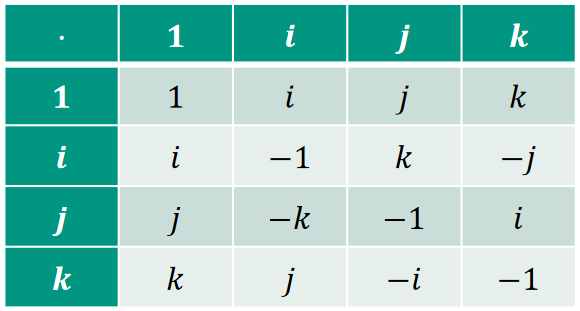
\includegraphics[width=0.35\textwidth]{images/quaternionen.png}
	\end{center}
	\item \textbf{Rechenoperationen}: Seien $\mathbf{q}=(a,\mathbf{u})^\top, \mathbf{r}=(b,\mathbf{v})^\top$ zwei Quaternionen
	\begin{itemize}
		\item \textbf{Addition}: $\mathbf{q}+\mathbf{r}=(a+b,\mathbf{u}+\mathbf{b})^\top$
		\item \textbf{Skalarprodukt}: $\langle \mathbf{q}\mid\mathbf{r}\rangle=a\cdot b+\langle \mathbf{v}\mid\mathbf{u}\rangle=a\cdot b+v_1\cdot u_1+v_2\cdot u_2+v_3\cdot u_3$
		\item \textbf{Multiplikation}: $\mathbf{q}\cdot\mathbf{r}=(a+u_1i+u_2j+u_3k)\cdot (b+v_1i+v_2j+v_3k)$
		\item \textbf{Konjugierte} Quaternion: $\mathbf{q^*}=(a,-\mathbf{u})^\top$
		\item \textbf{Norm}: $|\mathbf{q}|=\sqrt{\mathbf{q}\cdot\mathbf{q^*}}=\sqrt{\mathbf{q^*}\cdot\mathbf{q}}=\sqrt{a^2+u_1^2+u_2^2+u_3^2}$
		\item \textbf{Inverse}: $\mathbf{q}^{-1}=\cfrac{\mathbf{q^*}}{|\mathbf{q}|^2}$
	\end{itemize}
	\item \textbf{Einheitsquaternion} $\mathbb{S}^3=\{\mathbf{q}\in\HH\mid\lVert q \rVert^2=1\}$
	\item Beschreibung eines Vektors $\mathbf{p}\in\R^3$ als Quaternion $\mathbf{q}$: $\mathbf{q}=(0,\mathbf{p})^\top$
	\item Beschreibung eines Skalars $s\in\R^3$ als Quaternion $\mathbf{q}$: $\mathbf{q}=(s,\mathbf{0})^\top$
	\item Sei eine Rotation beschrieben durch eine Drehachse $\mathbf{a}$ mit $\mathbf{a}=1$ und einen Drehwinkel $\theta$, dann existiert hierfür eine Repräsentation als Quaternion: $\mathbf{q}=\left(\cos\frac{\theta}{2},\mathbf{a}\sin\frac{\theta}{2}\right)$
	\item Ein Punkt $\mathbf{v}$ wird mit einer Quaternion $\mathbf{q}$ rotiert durch:
	$\mathbf{v'}=\mathbf{qvq^{-1}}=\mathbf{qvq^{*}}$, wobei die letzte Gleichheit gilt, weil $\mathbf{q}$ ein Einheitsquaternion ist
	\item Verkettung von Rotationen $f\circ h$: $f(h(\mathbf{v}))=\mathbf{q}(\mathbf{rvr^*})\mathbf{q^*}$
\end{itemize}

\textit{Beispiel 1/72}\\

\textbf{Bewertung von Quaternionen}:
\begin{itemize}
	\item \textbf{Vorteile}: Kompakt, Anschaulich, Kein Gimbal Lock, Verkettung möglich, Stetige Repräsentation
	\item \textbf{Nachteil}: Nur Beschreibung von Rotation, keine Translation
\end{itemize}
\bigskip
\textbf{SLERP Interpolation}:
\begin{itemize}
	\item SLERP Interpolation von $\mathbf{q_1}$ nach $\mathbf{q_2}$ mit Parameter $t\in[0,1]$:	
	$$\text{SLERP}(\mathbf{q_1},\mathbf{q_2},t)=\frac{\sin((1-t)\cdot\theta)}{\sin\theta}\cdot\mathbf{q_1}+\frac{\sin(t\cdot\theta)}{\sin\theta}\cdot\mathbf{q_2}\qquad \text{mit }\langle\mathbf{q_1}\mid\mathbf{q_2}\rangle=\cos\theta$$
	\item Ergebnis: Rotation mit konstanter Winkelgeschwindigkeit
	\item \textbf{Problem}: Orientierungen in SO(3) werden durch Einheitsquaternionen doppelt abgedeckt, weil $\mathbf{q}$ und $-\mathbf{q}$ der gleichen Rotation entsprechen
	
	$\Rightarrow$ SLERP berechnet deshalb nicht immer die kürzeste Rotation. Es muss geprüft werden, ob die Rotation von $\mathbf{q_1}$ zu $\mathbf{q_2}$ oder $-\mathbf{q_1}$ zu $\mathbf{q_2}$ kürzer ist
\end{itemize}
\pagebreak
\textbf{Duale Quaternionen}:
\begin{itemize}
	\item Erlauben es auch Translationen zu berücksichtigen
	\item \textbf{Duale Zahlen} sind Zahlen der Form:
	$$d=p+\varepsilon\cdot s, \quad\text{wobei }\varepsilon^2=0$$ 
	mit \textbf{Primärteil} $p$, \textbf{Sekundärteil} $s$
	\item \textbf{Rechenoperationen}: Seien $d_1=p_1+\varepsilon\cdot s_1$ und $d_2=p_2+\varepsilon\cdot s_2$ duale Zahlen
	\begin{itemize}
		\item \textbf{Addition}: $d_1+d_2=p_1+p_2+\varepsilon\cdot(s_1+s_2)$
		\item \textbf{Multiplikation}: $d_1\cdot d_2=p_1\cdot p_2+\varepsilon\cdot(p_1\cdot s_2+p_2\cdot s_1)$
	\end{itemize}
	\item \textbf{Duale Quaternionen}: 
	$$DQ=(d_1,d_2,d_3,d_4), \qquad d_i=dp_i+\varepsilon\cdot ds_i$$
	\begin{itemize}
		\item Primärteil $dp_i$ enthält den Winkelwert $\theta/2$
		\item Sekundärteil $ds_i$ enthält die Translationsgröße $d/2$
	\end{itemize}
	\item \textbf{Multiplikationstabelle für duale Einheitsquaternionen}:
	\begin{center}
		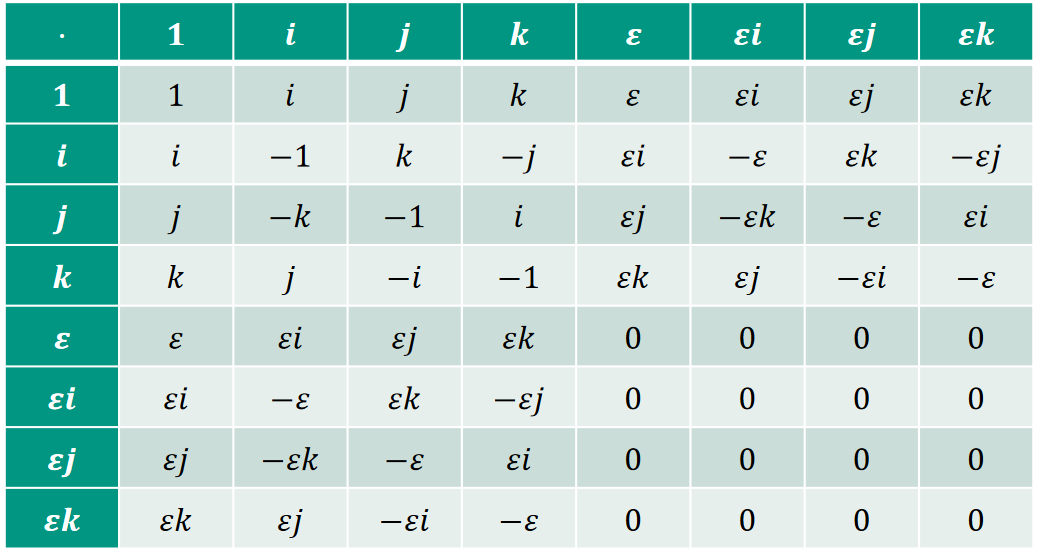
\includegraphics[width=0.7\textwidth]{images/duale-quaternionen.png}
	\end{center}
	\item Rotation um eine Achse $\mathbf{a}$ mit dem Winkel $\theta$: $\mathbf{q_r}=\left(\cos\frac{\theta}{2},\mathbf{a}\sin\frac{\theta}{2}\right)+\varepsilon\cdot(0,0,0,0)$
	\item Translation mit dem Vektor $\mathbf{t}=(t_x,t_y,t_z)$: $\mathbf{q_t}=(1,0,0,0)+\varepsilon\cdot(0,\frac{t_x}{2},\frac{t_y}{2},\frac{t_z}{2})$
	\item Kombination zu einer Transformation $T$: $\mathbf{q_T}=\mathbf{q_tq_r}$
	\item Eine Transformation $\mathbf{q_T}$ wird auf einen Punkt $\mathbf{p}$ als duale Quaternion wie folgt angewendet: $\mathbf{p'}=\mathbf{q_Tpq_T^*}, \text{mit }\mathbf{q_T^*}=(\mathbf{q_tq_r})^*=\mathbf{q_r^*q_t^*}$
	\item Konjugieren von $\mathbf{q}=\mathbf{p}+\varepsilon\cdot\mathbf{s}$: $\mathbf{q^*}=\mathbf{p^*}-\varepsilon\cdot\mathbf{s^*}$
\end{itemize}
\medskip
\textit{Beispiel 1/83-85}\\

\textbf{Bewertung von dualen Quaternionen}:
\begin{itemize}
	\item \textbf{Vorteile}: Erlauben Lagebeschreibung und Transformationen, Geringere Redundanz (nur 8 statt 12 Werte bei homogener Matrix)
	\item \textbf{Nachteile}: Lage durch Angabe einer Dualquaternion zu beschreiben ist relativ schwierig, Komplexe Verarbeitungsvorschriften 
\end{itemize}